\section{Setup}
\subsection{General Requirements}
\subsubsection{Hardware requirements}
The only hardware required is to own a CPU newer than a Pentium 4 with SSE2 instruction set.
\subsubsection{Software requirments}
This application can run on GNU/Linux on any distribution newer than Ubuntu 14.04, MacOs from 10.10 onward and Windows from 7 and onward;
Other than an operative system this application needs:
\begin{itemize}
    \item \textbf{Node.js}: to install it, the user can refer to the official web page nodejs.org for installation we recommend the LTS version;
    \item \textbf{npm}: Npm is the package manager that usually comes with Node.Js often, with a GNU/Linux distribution, the user needs to install npm as a separate package;
    \item \textbf{TypeScript}: to install TypeScript the user needs to run npm install typescript -g, the minimum version required is the 3.6.5;
    \item \textbf{ts-node}: to install ts-node the user needs need to run npm install ts-node -g, this operation will install globally the command ts-node;
\end{itemize}
For ease of use, the user can also install multiple packages in a single command.
\begin{center}
    \code{npm install typescript ts-node -g}
\end{center}
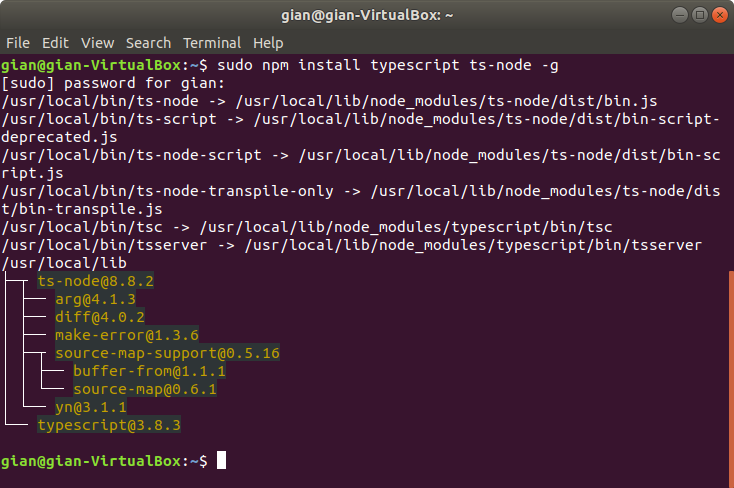
\includegraphics[width=\textwidth]{res/img/typescriptInstall.png}    



After entering the command the CLI should look like the picture.

\subsection{Etherless-cli}
\subsubsection{Requirements}
To develop with the unit test the user needs to install \textbf{mocha}
\begin{center}
    \code{npm install mocha -g}
\end{center}
This command will install mocha functionality globally.

\subsubsection{Setup}
To install Etherless-CLI is sufficient to start the installation process
\begin{center}
    \code{npm install -{}-dotenv-extended}
\end{center} 

To check if the setup completed correctly the user can run the unit test
\begin{center}
    \code{npm run test}
\end{center}

If the output of the command looks like the example than the installation was successful
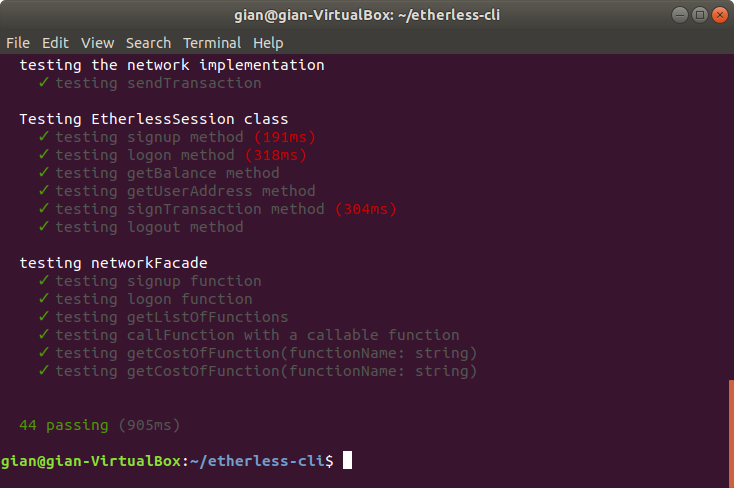
\includegraphics[width=\textwidth]{res/img/npmruntest.png}
Before using the software, the user needs to register to the Ethereum network or log in with an existing private key, after that, the user needs to add funds to the wallet that can be done through MetaMask importing the account.
\subsubsection{Run}
To run this program from the command line interface positioning on the main program folder
and type ts-node . <<command>> where <<command>> is the command that the user wants to run.
\subsection{Etherless-smart}
\subsubsection{Requirements}
To run correctly this component the user needs to install:
\begin{itemize}
    \item \textbf{Truffle}: to install Truffle the user needs to run \code{npm install Truffle -g};
    \item \textbf{Ganache-cli}: to install Ganache-cli the command to run is \code{npm install ganache-cli -g}.
\end{itemize}

\subsubsection{Setup}
\paragraph{Deploy on a local network}
Berfore the deploy starts the ganache server needs to be started on a separate terminal instance \code{ganache-cli}
\begin{itemize}
    \item \code{npm install -{}-dotenv-extended} : installs the package with all its dependencies;    
    \item \code{truffle build}:
    \item \code{truffle deploy -{}-network local}:
    \item \code{truffle test}: this command is optional an is for checking if the contract has been deployed correctly.
\end{itemize}
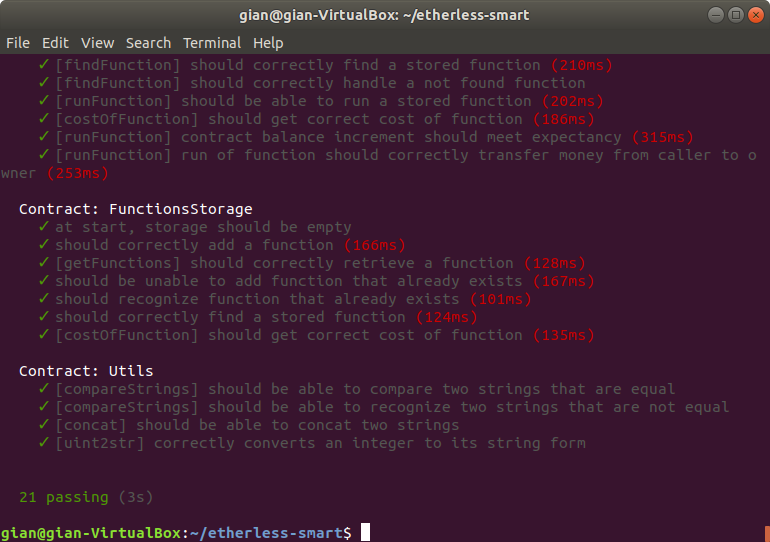
\includegraphics[width=\textwidth]{res/img/truffleTest.png}
\paragraph{Deploy on a production like envoirment}
Before the deploy on a network production like the user needs three different keys: an Etherscan API
key, and Infura API key and a private key from an Ethereum account with some founds.\\
After obtaining the credentials the user needs to edit the truffle-config.js file replacing the fields at the top with their own. \\
To deploy Etherless-smart in a production-like environment
by running the following commands from the component folder will install in the chosen network.
\begin{itemize}
    \item \code{npm install -{}-dotenv-extended} : installs the package with all its dependencies;
    \item \code{truffle build}: builds the smart contract to obtain the ABI file that is the Smart Contract representation;
    \item \code{truffle deploy -{}-network test}: deploys the compiled smart contract to the Ropsten test network;
    \item \code{truffle run verify EtherlessSmart -{}-network test}: confirms the Contract, this passage is needed for Etherscan to confirm the source code of the application, if the deploy is on a local network this command doesn't work;
\end{itemize}
After the deploy is a good practice to save the contract address somewhere safe, that will be needed to retrieve the contract.
\subsubsection{Run}
After the deploy, the contract will be always available and runnable through a web3 application like Remix with MetaMask injection ether in local that in a live network.
\subsection{Etherless-Server}
To run correctly this component the user needs to install:
\begin{itemize}
    \item \textbf{serverless}: to install serverless the user needs to run \code{npm install serverless -g}, this operation will install globally the commands serverless and sls;
    \item \textbf{mocha}: to install mocha the user needs to run \code{npm install mocha -g}, this operation will install globally the command mocha;
\end{itemize}
\subsubsection{Setup}
Before, the installation process the user needs to install the AWS credential on their
machine and register on the Serverless framework website that will handle the deploy and permission
management. After the registration on AWS and serverless to complete the setup by running
npm install on your local machine, when completed executing SLS deploy will upload to AWS.
\subsubsection{Run}
If the user completed the setup correctly run \code{serverless deploy} will upload the application to the lambda account and will be executable from the web.
